\documentclass{beamer}
\usepackage[utf8]{inputenc}

\usetheme{Madrid}
\usecolortheme{default}
\usepackage{txfonts}
\usepackage{listings}
\usepackage{adjustbox}
\usepackage{tabularx}
\usepackage{lmodern}
\usepackage{circuitikz}
\usepackage{tikz}

\usepackage{gvv}
\usepackage{cite}
\usepackage{amsmath,amssymb,amsfonts,amsthm}
\usepackage{algorithmic}
\usepackage{graphicx}
\usepackage{textcomp}
\usepackage{xcolor}
\usepackage{txfonts}
\usepackage{listings}
\usepackage{enumitem}
\usepackage{mathtools}
\usepackage{gensymb}
\usepackage{comment}
\usepackage{tkz-euclide} 
\usepackage{listings}                                      
\def\inputGnumericTable{}                                
\usepackage{color}                                            
\usepackage{array}                                            
\usepackage{longtable}
\usepackage{multicol}
\usepackage{calc}                                             
\usepackage{multirow}                                         
\usepackage{hhline}                                           
\usepackage{ifthen}

\setbeamertemplate{page number in head/foot}[totalframenumber]

\usepackage{tcolorbox}
\tcbuselibrary{minted,breakable,xparse,skins}



\definecolor{bg}{gray}{0.95}
\DeclareTCBListing{mintedbox}{O{}m!O{}}{%
  breakable=true,
  listing engine=minted,
  listing only,
  minted language=#2,
  minted style=default,
  minted options={%
    linenos,
    gobble=0,
    breaklines=true,
    breakafter=,,
    fontsize=\small,
    numbersep=8pt,
    #1},
  boxsep=0pt,
  left skip=0pt,
  right skip=0pt,
  left=25pt,
  right=0pt,
  top=3pt,
  bottom=3pt,
  arc=5pt,
  leftrule=0pt,
  rightrule=0pt,
  bottomrule=2pt,
  toprule=2pt,
  colback=bg,
  colframe=orange!70,
  enhanced,
  overlay={
    \begin{tcbclipinterior}
    \fill[orange!20!white] (frame.south west) rectangle ([xshift=20pt]frame.north west);
    \end{tcbclipinterior}},
  #3,
}
\lstset{
    language=C,
    basicstyle=\ttfamily\small,
    keywordstyle=\color{blue},
    stringstyle=\color{orange},
    commentstyle=\color{green!60!black},
    numbers=left,
    numberstyle=\tiny\color{gray},
    breaklines=true,
    showstringspaces=false,
}

\title 
{5.8.29}
\date{October 12, 2025}


\author 
{Sai Sreevallabh - EE25BTECH11031}



\begin{document}


\frame{\titlepage}
\begin{frame}{Question}
$2$ women and $5$ men can together finish an embroidery work in $4$ days, while $3$ women and $6$ men can finish it in $3$ days. Find the time taken by $1$ women alone to finish the work, and also that taken by $1$ man alone.\\
\end{frame}



\begin{frame}{Theoretical Solution}
Let the fraction of work done by a woman in a day be $x$ and the fraction of work done by a man in a day be $y$, represented as 
\begin{align}
    \vec{x} = \myvec{x\\y}
\end{align}

Also, if $a$ days are taken for a work to complete, the fraction of work completed in a single day is $\frac{1}{a}$.

\end{frame}

\begin{frame}{Theoretical Solution}

Using the above, we can write the given data into two equations:

\begin{align}
    \myvec{2&5}\vec{x} = \frac{1}{4} \label{eq2}
\end{align}

\begin{align}
    \myvec{3&6}\vec{x} = \frac{1}{3} \label{eq3}
\end{align}
\end{frame}

\begin{frame}{Theoretical Solution}
Converting into Reduced Row Echelon Form:

\begin{align}
    \augvec{2}{1}{2&5&\frac{1}{4}\\[1ex]3&6&\frac{1}{3}}
    \xleftrightarrow[]{R_1\xrightarrow{}\frac{1}{2}R_1} 
    \augvec{2}{1}{1&\frac{5}{2}&\frac{1}{4}\\[1ex]3&6&\frac{1}{3}}
\end{align}

\begin{align}
    \augvec{2}{1}{1&\frac{5}{2}&\frac{1}{4}\\[1ex]3&6&\frac{1}{3}}
    \xleftrightarrow[]{R_2\xrightarrow{}R_2-3R_1}
    \augvec{2}{1}{1&\frac{5}{2}&\frac{1}{4}\\[1ex]0&-\frac{3}{2}&-\frac{1}{24}}
\end{align}
\end{frame}

\begin{frame}{Theoretical Solution}
    \begin{align}
    \augvec{2}{1}{1&\frac{5}{2}&\frac{1}{4}\\[1ex]0&-\frac{3}{2}&-\frac{1}{24}}
    \xleftrightarrow[]{R_2\xrightarrow{}-\frac{2}{3}R_2}
    \augvec{2}{1}{1&\frac{5}{2}&\frac{1}{4}\\[1ex]0&1&\frac{1}{36}}
\end{align}

\begin{align}
    \augvec{2}{1}{1&\frac{5}{2}&\frac{1}{4}\\[1ex]0&1&\frac{1}{36}}
    \xleftrightarrow[]{R_1\xrightarrow{}R_1-\frac{5}{2}R_2}
    \augvec{2}{1}{1&0&\frac{1}{18}\\[1ex]0&1&\frac{1}{36}}
\end{align}
\end{frame}

\begin{frame}{Theoretical Solution}
    We get
\begin{align}
    \vec{x} = \myvec{\frac{1}{18}\\[1ex]\frac{1}{36}}
\end{align}\\

The number of days can be written as
\begin{align}
    \frac{1}{y} = 36 \ \  \text{and} \ \ \frac{1}{x} = 18
\end{align}\\

$\therefore$ The time taken by one woman alone to finish the work is $18$ days, and the time taken by one man alone to finish the work is $36$ days.\\
\end{frame}



\begin{frame}[fragile]
    \frametitle{C Code - Solving Using Gaussian Elimination}

    \begin{lstlisting}
#include <stdio.h>

void Solve_Gaussian(double A[3], double B[3], double sol[2]) {
    // If A[0] == 0, swap rows to avoid division by zero
    //Also covers the case where the matrix is diagonal.
    if (A[0] == 0) {
        for (int i = 0; i < 3; i++) {
            double temp = A[i];
            A[i] = B[i];
            B[i] = temp;
        }
    }

    \end{lstlisting}

\end{frame}

\begin{frame}[fragile]
    \frametitle{C Code - Solving Using Gaussian Elimination}

    \begin{lstlisting}
    
    double factor = B[0] / A[0];
    for (int i = 0; i < 3; i++) {
        B[i] = B[i] - factor * A[i];
    }

    sol[1] = B[2] / B[1];
    sol[0] = (A[2] - A[1] * sol[1]) / A[0];
}

    \end{lstlisting}

\end{frame}

\begin{frame}[fragile]
    \frametitle{Python Code - Using Shared Object}
    \begin{lstlisting}
import ctypes
import numpy as np
import matplotlib.pyplot as plt

c_lib = ctypes.CDLL("./code.so")

c_lib.Gaussian.argtypes = [ctypes.c_double*3, ctypes.c_double*3, ctypes.c_double*2]

A = (ctypes.c_double*3)(2,5,1.0/4.0)
B = (ctypes.c_double*3)(3,6,1.0/3.0)

sols = (ctypes.c_double*2)(0.0,0.0)

c_lib.Gaussian(A,B,sols)



\end{lstlisting}
\end{frame}

\begin{frame}[fragile]
    \frametitle{Python Code - Using Shared Object}
    \begin{lstlisting}

sols[0] = np.round(sols[0],3)
sols[1] = np.round(sols[1],3)

plt.plot([-2,2], [0.85,-0.75], c='green', label = r"$2x+5y=\frac{1}{4}$")
plt.plot([-2,2], [19/18,-17/18], c='blue', label = r"$3x+6y=\frac{1}{3}$")

plt.scatter(sols[0],sols[1])

plt.annotate(
        f"{sols[0],sols[1]}",
        xy=(sols[0],sols[1]),
        xytext = (2,2),
        textcoords = "offset points"
        )

\end{lstlisting}
\end{frame}

\begin{frame}[fragile]
    \frametitle{Python Code - Using Shared Object}
    \begin{lstlisting}
    
ax = plt.gca()
ax.spines['top'].set_color('none')
ax.spines['bottom'].set_position('zero')
ax.spines['right'].set_color('none')
ax.spines['left'].set_position('zero')
plt.xlabel('x')
plt.ylabel('y')
plt.legend(loc='best')
plt.grid()
plt.axis('equal')

plt.savefig("../Figs/plot(py+C).png")
plt.show()

\end{lstlisting}
\end{frame}


\begin{frame}{Plot-Using Both C and Python}
    \centering
    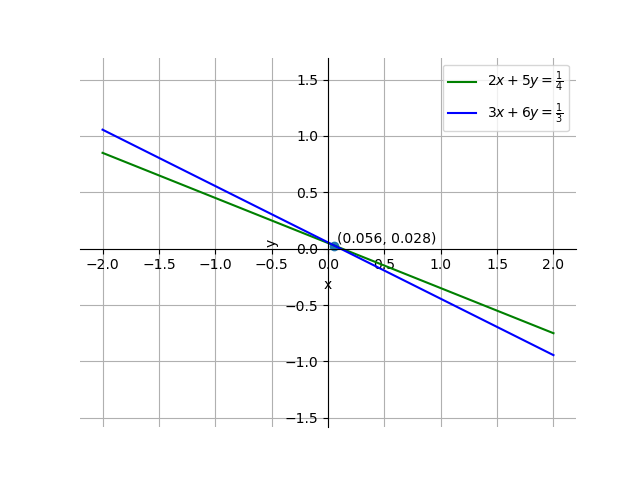
\includegraphics[width=\columnwidth, height=0.8\textheight, keepaspectratio]{Figs/plot(py+C).png}     
\end{frame}

%-------End of Python+C-------------


\begin{frame}[fragile]
    \frametitle{Python Code}
    \begin{lstlisting}
import numpy as np
import matplotlib.pyplot as plt
import numpy.linalg as LA

M = np.array([[2,5],
              [3,6]])
b = np.array([1/4,1/3])
x = LA.solve(M, b)


plt.scatter(x[0],x[1])

x[0]=np.round(x[0],3)
x[1]=np.round(x[1],3)



\end{lstlisting}
\end{frame}

\begin{frame}[fragile]
    \frametitle{Python Code}
    \begin{lstlisting}

plt.plot([-2,2], [0.85,-0.75], c='red', label = r'$2x+5y=\frac{1}{4}$')
plt.plot([-2,2], [19/18,-17/18], c='black', label = r'$3x+6y=\frac{1}{3}$')

plt.annotate(
        f'{x[0],x[1]}',
        xy=(x[0],x[1]),
        xytext = (2,2),
        textcoords = "offset points"
        )


\end{lstlisting}
\end{frame}

\begin{frame}[fragile]
    \frametitle{Python Code}
    \begin{lstlisting}

ax = plt.gca()
ax.spines['top'].set_color('none')
ax.spines['bottom'].set_position('zero')
ax.spines['right'].set_color('none')
ax.spines['left'].set_position('zero')
plt.xlabel('x')
plt.ylabel('y')
plt.legend(loc='best')
plt.grid()
plt.axis('equal')

plt.savefig("../Figs/plot(py).png")
plt.show()


    \end{lstlisting}
\end{frame}


\begin{frame}{Plot-Using Python only}
    \centering
    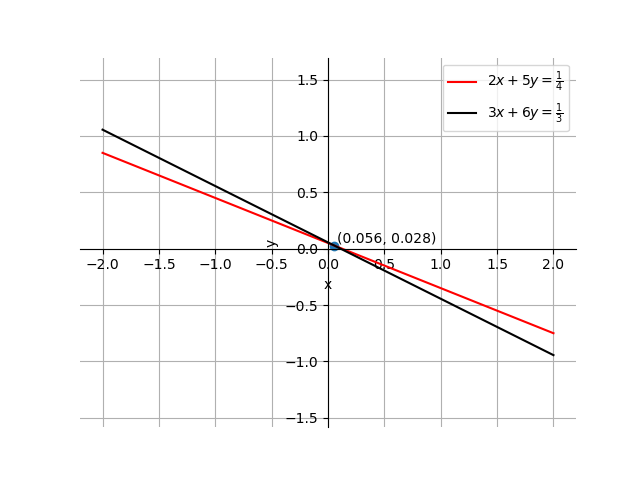
\includegraphics[width=\columnwidth, height=0.8\textheight, keepaspectratio]{Figs/plot(py).png}     
\end{frame}


\end{document}
